\chapter{Metodologia}

\section{Abordagem de pesquisa:}
Levando em conta que o presente trabalho possui como objetivo realizar avaliação automática de respostas dissertativas, pretende-se que o resultado final do mesmo seja uma proposta de resolução desse problema. Assim, podemos classificar sua abordagem de metodologia como experimental, haja vista que serão realizados experimentos com os dados e as técnicas, que serão descritas no decorrer do texto, afim de atingir o objetivo proposto.

%O presente trabalho possui a abordagem exploratória, haja vista que, desejamos avaliar o desempenho de diferentes técnicas de NLP para avaliação de um grau de parafraseamento entre as respostas. Afim de obter uma clareza maior em que técnicas podem ter um melhor desempenho no trabalho de avaliar questões dissertativas. 

%Em relação ao método, podemos encaixar o estudo como um estudo de corte, pois serão analisados quais parâmetros contidos nos textos podem influenciar na similaridade semântica de seu conteúdo com o texto de referência. Também podemos relacionar nosso estudo com estudos de caso, já que alguns dos dados utilizados serão específicos de exames realizados no Centro Universitário FEI, o que gerará uma compreensão de quais variáveis influenciaram o resultado e detalhes específicos do caso que podem ser relevantes para o caso.

\section{Bases de dados:}
Como fonte principal de dados, utilizaremos o \textit{DataSet ASQA (Answer Summaries for Questions which are Ambiguous)} da \textit{Google Research} em parceria com as universidade de \textit{Duke University} e \textit{Cornell University}, o \textit{DataSet} contém respostas dissertativas para questões com perguntas ambíguas, isso permitirá a construção dos experimentos e refino das técnicas que serão utilizadas no presente trabalho \cite{dataSetGoogleASQA}.


Além da fonte principal de dados, planejamos também utilizar dados das respostas dissertativas dos alunos de Ciência da Computação do Centro Universitário FEI para questões dissertativas do ENADE.

Ademais, existe a possibilidade de que um futuro questionário seja confeccionado para que, com a ajuda voluntária dos alunos da mesma instituição, mais dados sejam coletados e usados no presente trabalho. Essa possibilidade será investigada caso seja necessário.

%Faremos uso de uma base de dados própria fornecida pela Professora Leila Bergamasco, a base contém as respostas dissertativas das questões de um simulado do ENADE, constam apenas respostas de alunos do Centro Universitário FEI, integrantes do curso de Ciência da Computação entre o 5° e 8° ciclo. Ademais, 

\section{Materiais:}
Serão utilizados computadores para o desenvolvimento da experimentação e a documentação do processo. Os computadores principais utilizados serão de posse própria, caso seja necessário, também podem ser utilizados computadores disponibilizados no campus do Centro Universitário FEI. 

Se no decorrer do processo de experimentação, dificuldades em relação as capacidades de processamento e memórias dos computadores forem identificados, abre-se também a possibilidade do uso de plataformas disponibilizadas \textit{online}, como o \textit{Google Colab} (\url{https://colab.google/}) e a \textit{Weights \& Biases} (\url{https://wandb.ai/site/}), ambas oferecem possibilidade de uso gratuito para estudantes que utilizarem apenas com fins acadêmicos.

\section{Métodos:}
Serão utilizados métodos de NLP, tais como mineração de texto, medição de distância de cossenos (para mensurar similaridade de textos), frequência de sentidos de palavras (SFD), presença de palavras-chaves (KW), ordem de sequência das palavras, entre outros. Para compor toda a metodologia, pretende-se elaborar uma métrica de avaliação do grau de similaridade semântica entre dois conteúdos. 

Assumindo que dois textos possuem exatamento o mesmo conteúdo, sua similaridade poderia ser descrita em uma escala percentual como 100\%, por outro lado, haverão textos que possuirão conteúdo sintaticamente diferentes, logo, espera-se que seu percentual de similaridade diminua, porém, ainda assim seria possivel a existência de similaridade semântica entre esse texto e a respota correta, sendo assim, é importante avaliar aspectos semânticos do texto. 

Desta forma, a hipótese é que, para avaliarmos tal similaridade, será necessário avaliar uma série de fatores importantes que irão compor a métrica de avaliação proposta. Esses fatores seriam:
\begin{itemize}
    \item \textbf{As propriedades da sintaxe do texto:} Tal fator será levado em consideração tendo em vista que os trabalhos avaliados na revisão bibliográfica demonstraram a importância de propriedades sintáticas como a ordem em que as sequências de palavras estão posicionadas no texto.
    \item \textbf{Frequência de Sentidos de Palavras (SFD):} Pois também foi demonstrado nos trabalhos avaliados na revisão bibliográfica que essa medida estatística é relevante para a avaliação das respostas.
    \item \textbf{A medição da distância de cossenos:} Essa medida tem relevância para a métrica pois mensura a similaridade semântica entre dois textos através de suas representações vetoriais.
    \item \textbf{A presença de palavras-chave (\textit{keywords}):} Serão palavras definidas para cada questão pelo seu confeccionador como termos com um grau mais elevado de relevância para a resposta esperada do aluno. determinadas como parte da resposta padrão para aquela questão.
\end{itemize}

Todos os fatores apresentados acima já foram utilizados de maneira isolada por diferentes trabalhos como uma forma de avaliação. No caso do presente trabalho pretende-se realizar uma junção dos fatores em uma métrica única para avaliação, averiguando-se ao longo do desenvolvimento do trabalho qual a relevância de cada um deles, para que um peso ajustado seja atribuído para cada fator da métrica. 

Caso a métrica proposta acima apresente bons resultados, pode-se cogitar a elaboração de uma segunda métrica, em que dois outros fatores seriam adicionados como uma possível melhoria à primeira, sendo eles: 
\begin{itemize}
    \item A verificação da possibilidade de um texto ser classificado como paráfrase de outro, já que o trabalho possui como hipótese que toda resposta correta é em algum grau uma paráfrase da resposta modelo. Com a identificação da paráfrase, como pode ser feita a medição do grau de parafraseamento entre os dois textos.
    \item A quantidade de modificações necessárias para que a resposta fornecida seja transformada lexicalmente e sintaticamente na resposta modelo.
\end{itemize}
Esses dois fatores não foram considerados nos trabalhos revisados anteriormente, na eventual proposta de uma segunda métrica, ter-se-á como hipótese que os dois fatores resultarão em uma melhoria no resultado.

A proposta da métrica pode ser matemáticamente descrita como na Equação 2, que contém a equação de uma média ponderada.
\begin{equation}
Métrica1 = \frac{fator1 \times peso_{1} + fator2 \times peso_{2} + fator3 \times peso_{3} + fator4 \times peso_{4}}{\sum_{i=1}^{4}peso_{i}}
\end{equation}

Em que \textit{fator1} são as propriedades sintáticas do texto, o \textit{fator2} representa o SFD, o \textit{fator3} é a distância de cossenos e o \textit{fator4} é referente as \textit{keywords}. 

Como resultado a métrica deverá fornecer um número no intervalo de 0  100 que, quanto maior, indica maior proximidade semântica entre os textos e uma maior probabilidade de acerto da resposta fornecida por um aluno. 

No caso da segunda métrica, o diferencial seria adição dos dois outros fatores para mensurar o grau de parafraseamento e a quantidade de modificações, sendo respectivamente o \textit{fator5} e o \textit{fator6} como descrito na Equação 3.

\begin{equation}
\tiny Métrica2 = \frac{fator1 \times peso_{1} + fator2 \times peso_{2} + fator3 \times peso_{3} + fator4 \times peso_{4} + fator5 \times peso_{5} + fator6 \times peso_{6}}{\sum_{i=1}^{6}peso_{i}}
\end{equation}

\section{Avaliação:}
Para avaliação do desempenho das técnicas propostas, as bases de dados serão divididas em duas, uma primeiramente para treinamento e refino dos experimentos. Após os resultados estarem satisfatórios, a segunda parte dos dados será utilizada para a validação dos resultados obtidos pelo algoritmo, verificando se estão condizente com os resultados fornecidos pelas avaliações registradas nos dados e se seu funcionamento é geral ou se há algum viés nos resultados. Uma representação visual das etapas gerais imaginadas para o processo pode ser vista na Figura \ref{figure:4}.

\begin{figure}[h!]
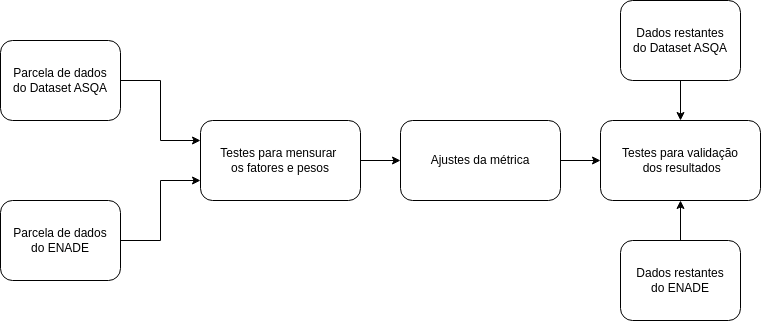
\includegraphics[width=\textwidth]{./imgs/diagramasTcc.png}
\caption{Diagrama geral das etapas do processo.}\label{figure:4}
\end{figure}

% olhar depois:

% https://www.researchgate.net/publication/337412528_Avaliacao_Automatica_de_respostas_discursivas_curtas_baseado_em_tres_dimensoes_linguisticas

% https://revistas.unoeste.br/index.php/ce/article/view/4595

% https://physionet.org/content/radqa/1.0.0/

% https://ppgee.propesp.ufpa.br/ARQUIVOS/teses/tese_abntex_final.pdf

% dataset search google

\newpage